\chapter{Modelo de Interaccion}
 
En este capitulo mostramos las interfaces con las que se van a implementar el sistema, estas pantallas y interfaces diseñadas son directamente en código HTML, para poder adelantar un poco a la implementación. 
Estas interfaces se utilizan para poder facilitar el entendimiento de la especificación de los requerimientos explicada con casos de uso.


\begin{figure}[htbp!]
	\begin{center}
	Interfaz de Usuario IU0:Login
	Interfaz necesaria para acceder al sistema.
		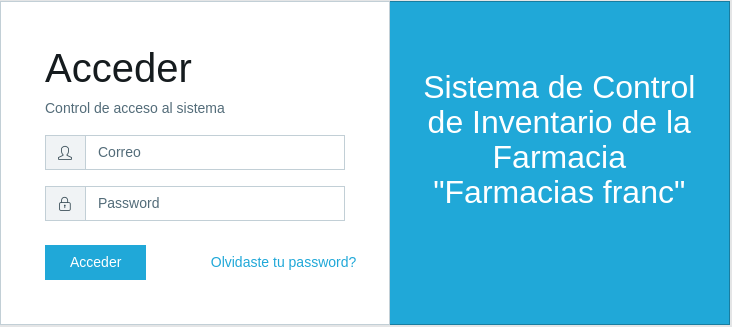
\includegraphics[width=\textwidth]{Pantallas/login}
		\caption{Modelo de interacción}
	\end{center}
\end{figure}



\begin{figure}[htbp!]
	\begin{center}
	
Primera pantalla que muestra el sistema apenas el Empleado o Dueño accede al sistema
		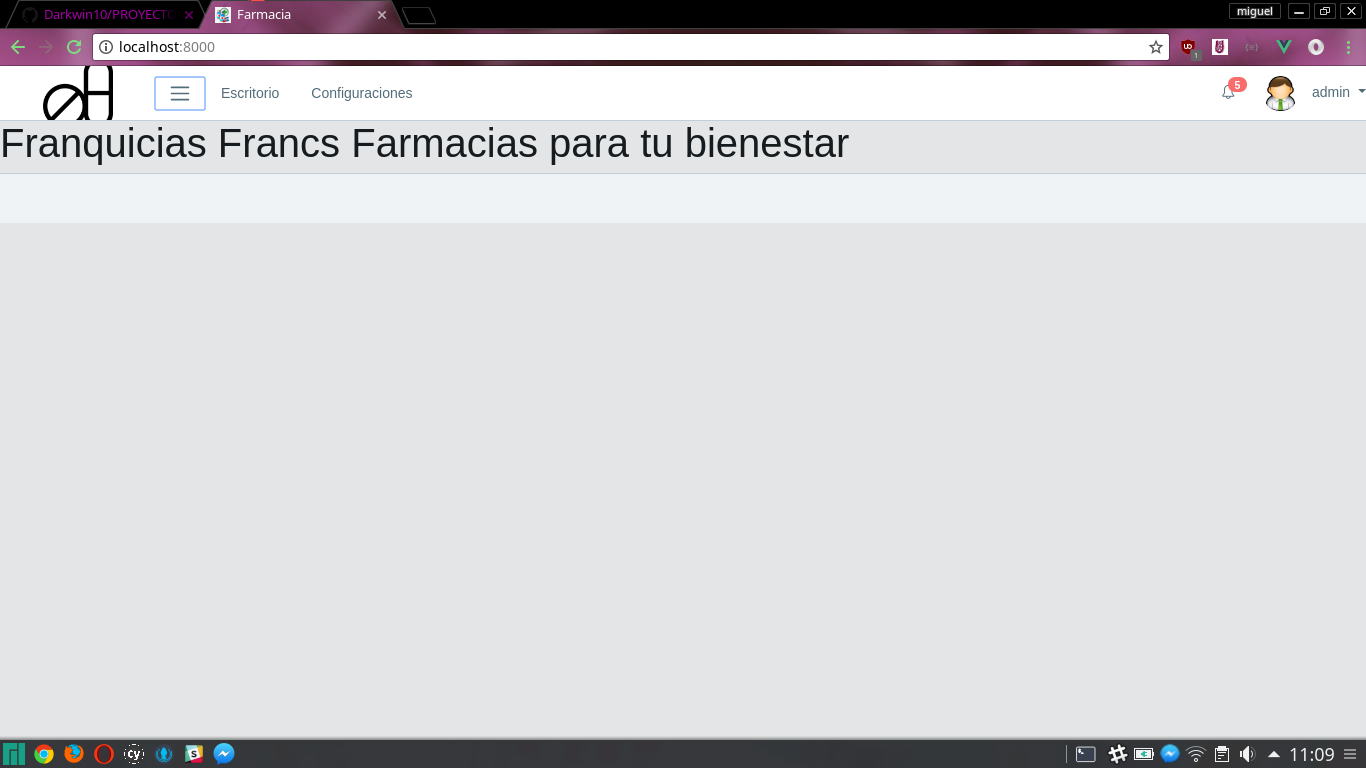
\includegraphics[width=\textwidth]{Pantallas/PantallaPrincipal}
		\caption{Interfaz de Usuario IU1:Pantalla Principal}
	\end{center}
\end{figure}






\begin{figure}[htbp!]
	\begin{center}
	\subsection{Formularios}
	pantallas para mostrar los datos requeridos para agregar un nuevo elemento
y también pantallas que se muestran para actualizar un elemento 
con la diferencia de que los datos estarán llenos.
		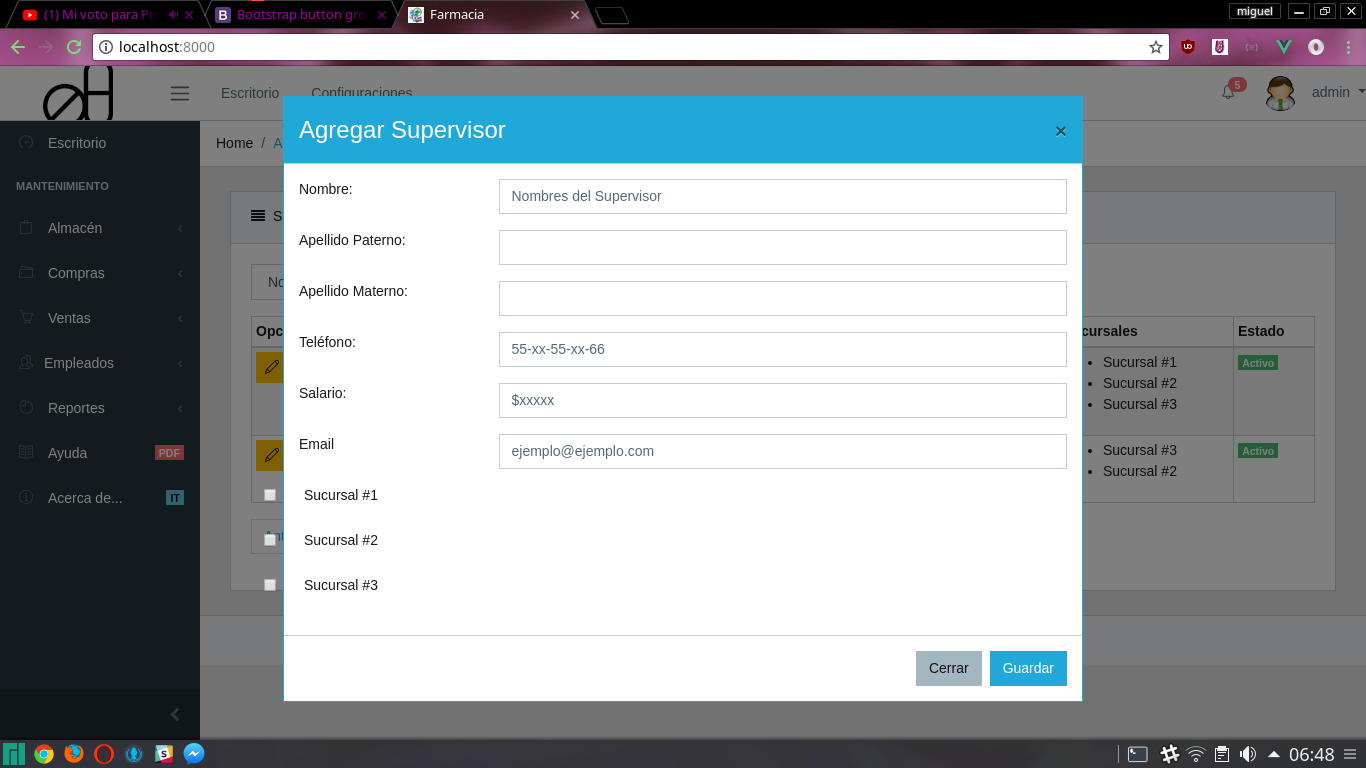
\includegraphics[width=\textwidth]{Pantallas/FormularioSupervisor}
		\caption{Interfaz de Usuario IU2:Formulario Supervisor}
	\end{center}
\end{figure}




\begin{figure}[htbp!]
	\begin{center}
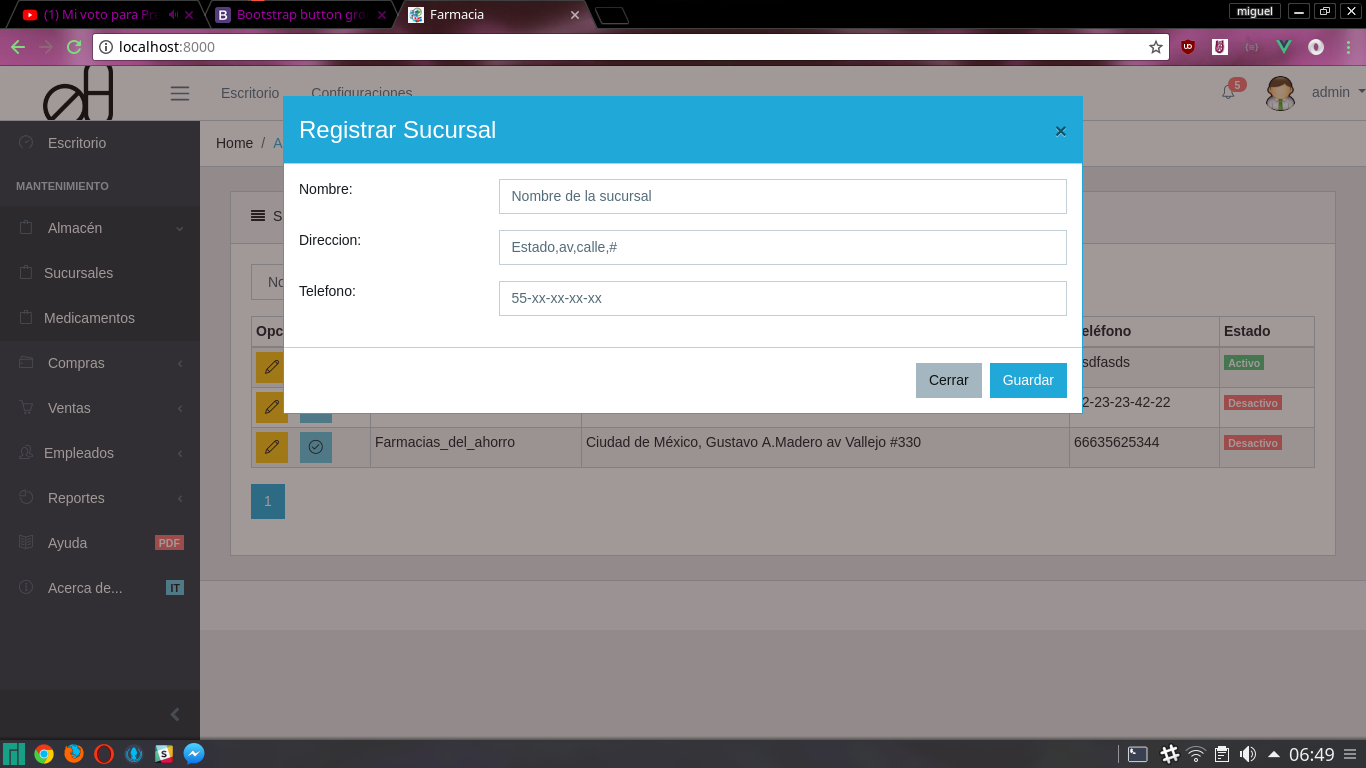
\includegraphics[width=\textwidth]{Pantallas/FormularioSucursal}
		\caption{Interfaz de Usuario IU3: Formulario Sucursal}
	\end{center}
\end{figure}



\begin{figure}[htbp!]
	\begin{center}
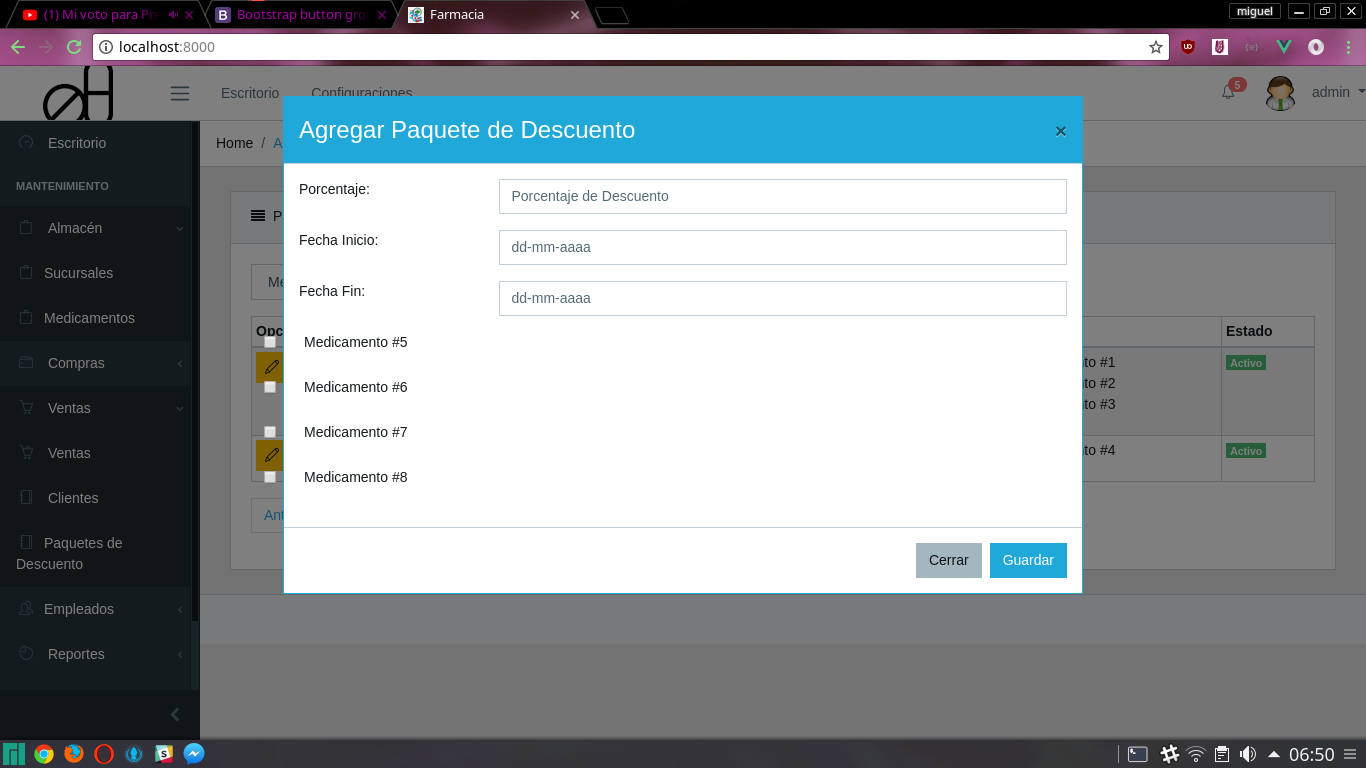
\includegraphics[width=\textwidth]{Pantallas/FormularioPaqueteDescuento}
		\caption{Interfaz de Usuario IU4: Formulario Paquete de Descuento}
	\end{center}
\end{figure}





\begin{figure}[htbp!]
	\begin{center}
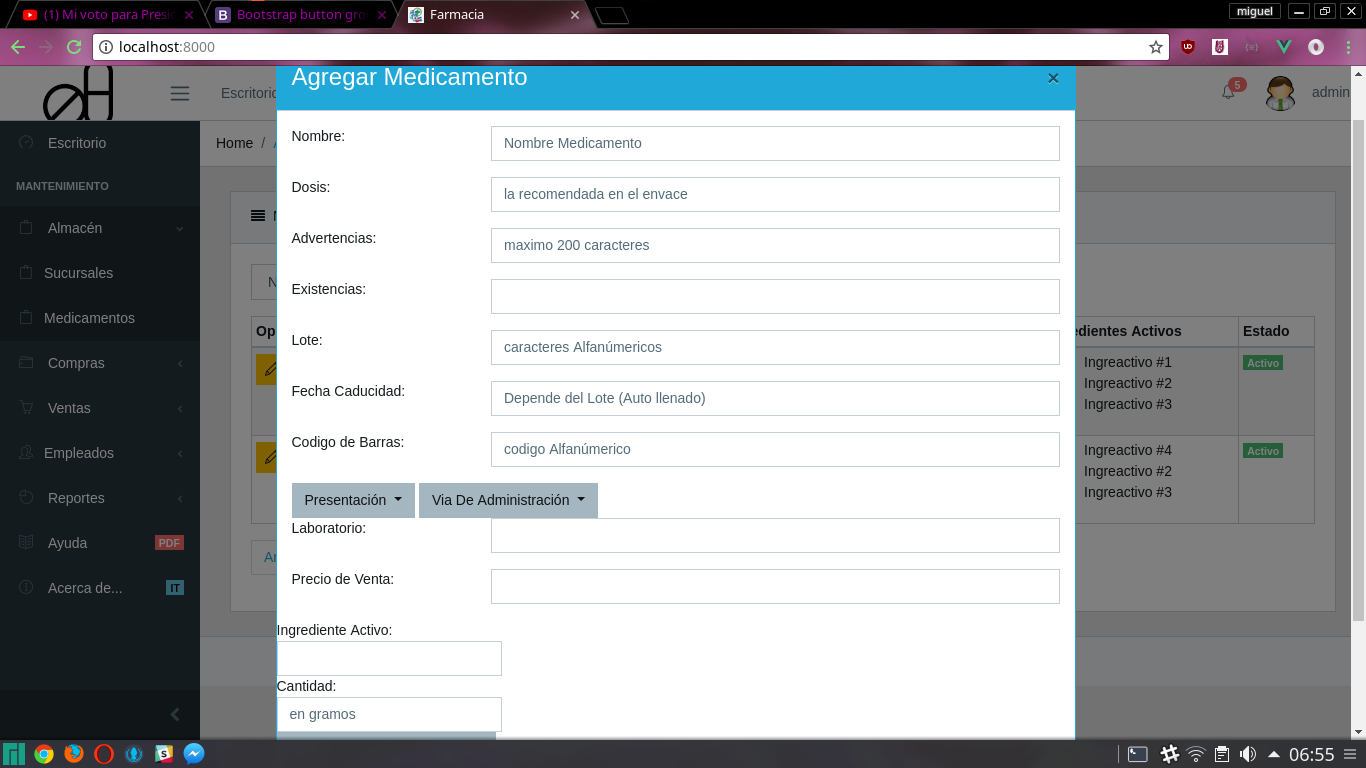
\includegraphics[width=\textwidth]{Pantallas/FormularioMedicamento}
		\caption{Interfaz de Usuario IU5: Formulario Medicamento}
	\end{center}
\end{figure}



\begin{figure}[htbp!]
	\begin{center}
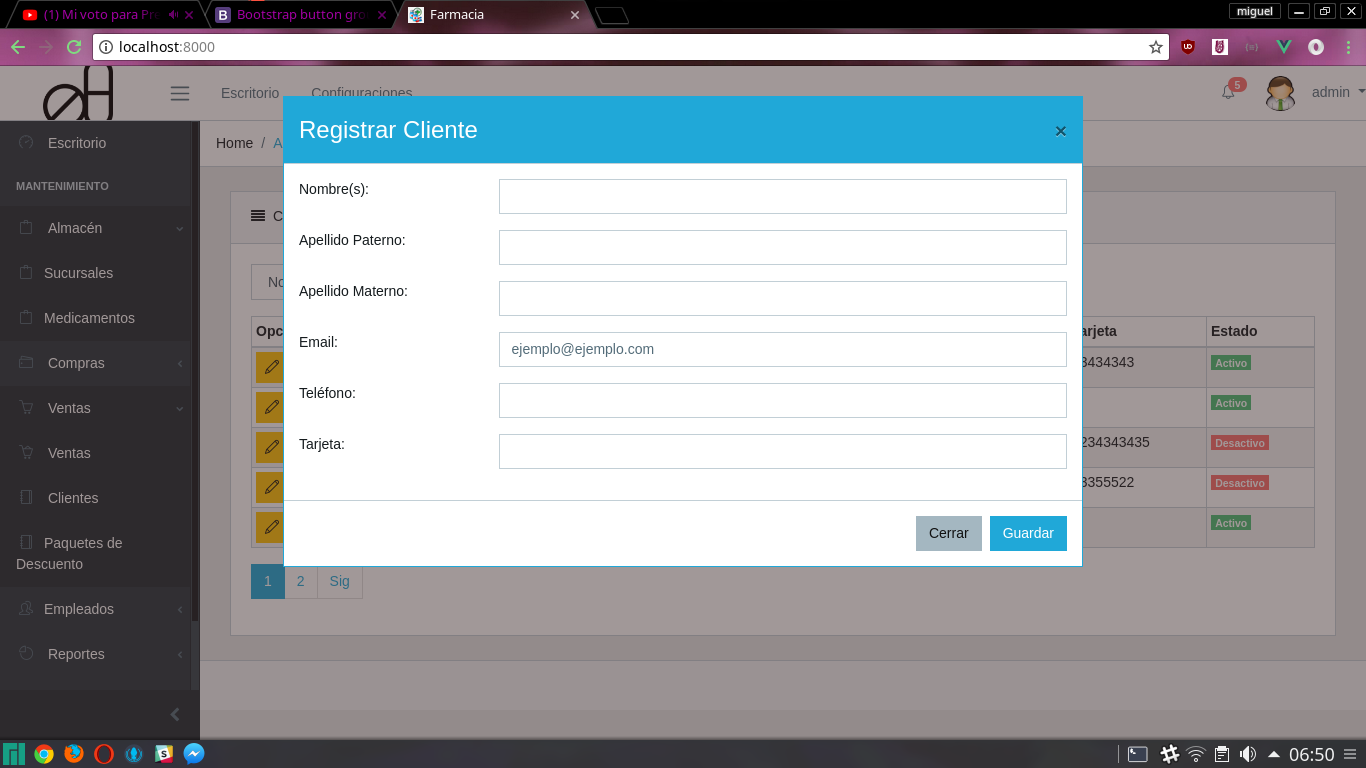
\includegraphics[width=\textwidth]{Pantallas/FormularioClientes}
		\caption{Interfaz de Usuario IU6: Formulario Cliente}
	\end{center}
\end{figure}


\begin{figure}[htbp!]
	\begin{center}
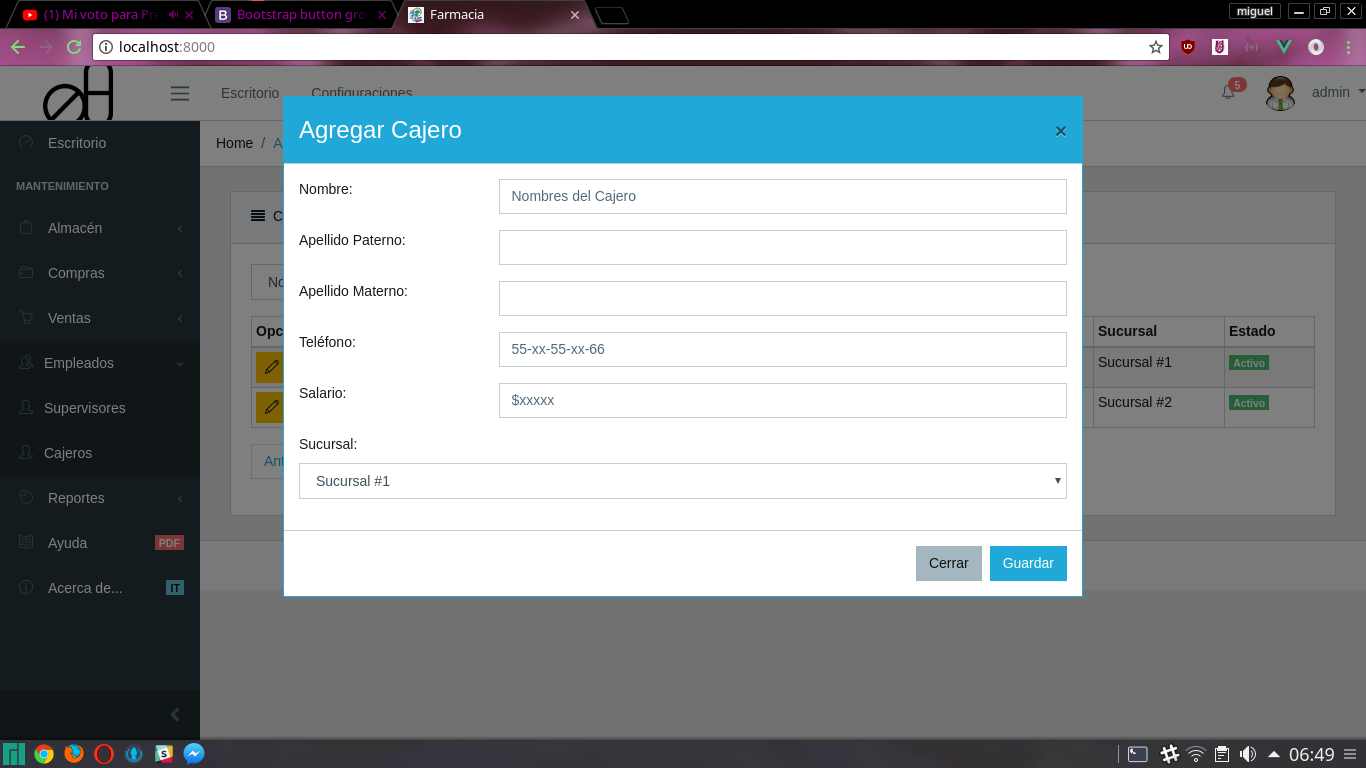
\includegraphics[width=\textwidth]{Pantallas/FormulariCajero}
		\caption{Interfaz de Usuario IU7:Formulario Cajero}
	\end{center}
\end{figure}



\begin{figure}[htbp!]
	\begin{center}
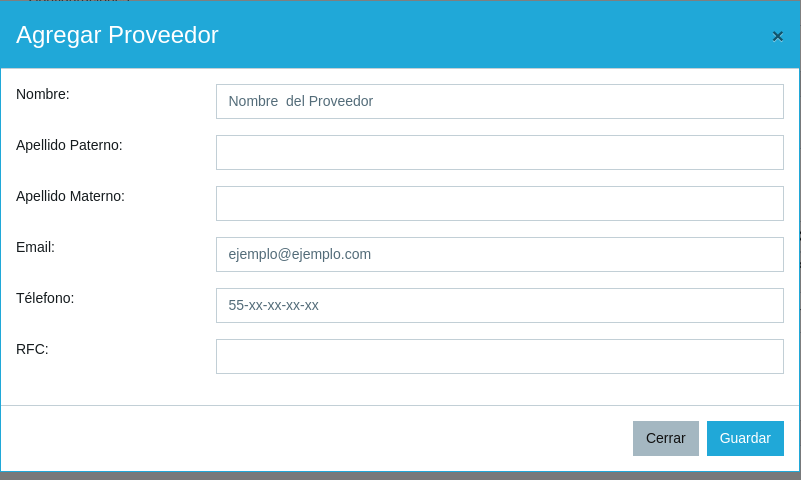
\includegraphics[width=\textwidth]{Pantallas/ProveedorFormulario}
		\caption{Interfaz de Usuario IU8:Formulario Proveedor}
	\end{center}
\end{figure}


\begin{figure}[htbp!]
	\begin{center}
	 \subsection{Botones}
	Botones para editar, desactivar y activar un elemento.

\includegraphics[width=\textwidth]{Pantallas/bottonDesactivar}
		\caption{Interfaz de Usuario IU9:Botón desactivar}
	\end{center}
\end{figure}



\begin{figure}[htbp!]
	\begin{center}

\includegraphics[width=\textwidth]{Pantallas/bottonActivar}
		\caption{Interfaz de Usuario IU10:Botón activar}
	\end{center}
\end{figure}



\begin{figure}[htbp!]
	\begin{center}

\includegraphics[width=\textwidth]{Pantallas/botonEditar}
		\caption{Interfaz de Usuario IU11:Botón editar}
	\end{center}
\end{figure}




\begin{figure}[htbp!]
	\begin{center}
	En ocasiones El empleado o incluso el propio dueño pueda olvidar su contraseña.
En estos casos sera necesario proporcionar una medida rápida para entrar al sistema .esta es la Interfaz que se muestra para recuperar la contraseña.
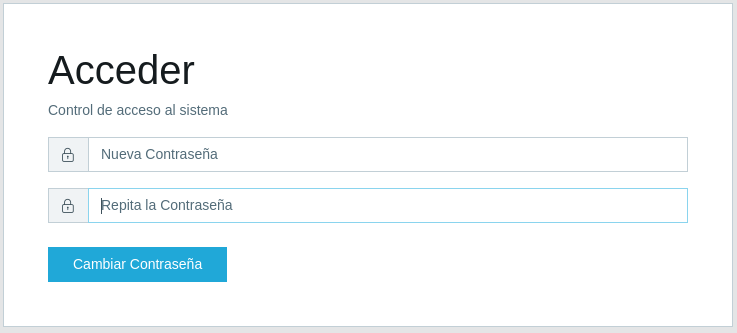
\includegraphics[width=\textwidth]{Pantallas/RecuperarContra}
		\caption{Interfaz de Usuario IU12:Recuperar Contraseña}
	\end{center}
\end{figure}




\begin{figure}[htbp!]
	\begin{center}
	\subsection{Tablas}
En estas Interfaces se muestran las tablas con los respectivos datos en formato
de tabla, donde también hay una columna extra aparte de los atributos que tiene el elemento, que muestra las opciones que se tienen para interactuar con los datos
del elemento. En el caso de que el elemento sea Medicamentos, no se muestran todos los atributos ya que son demasiados,por eso en la columna de opciones tiene una opción para ver los demás atributos en la tabla.
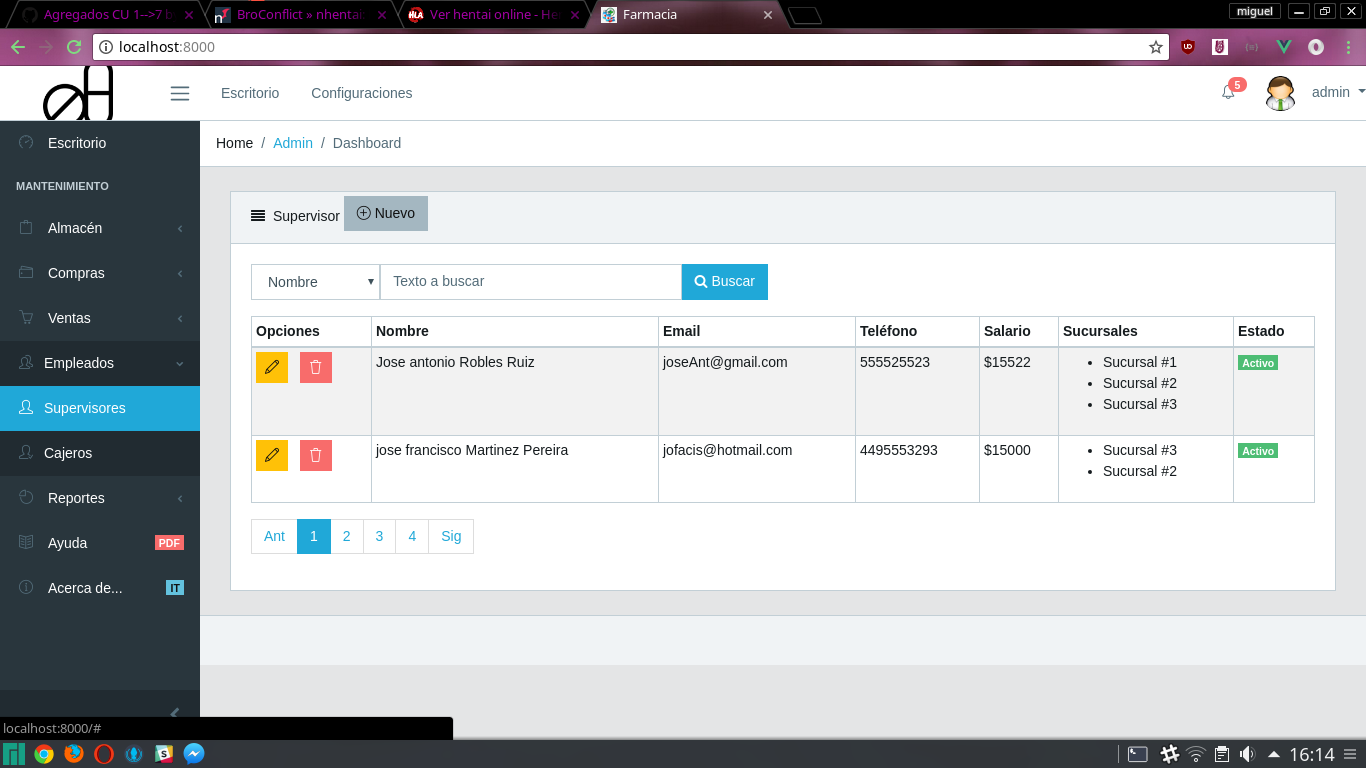
\includegraphics[width=\textwidth]{Pantallas/tablaSupervisores}
		\caption{Interfaz de Usuario IU13:Tabla supervisores.}
	\end{center}
\end{figure}




\begin{figure}[htbp!]
	\begin{center}
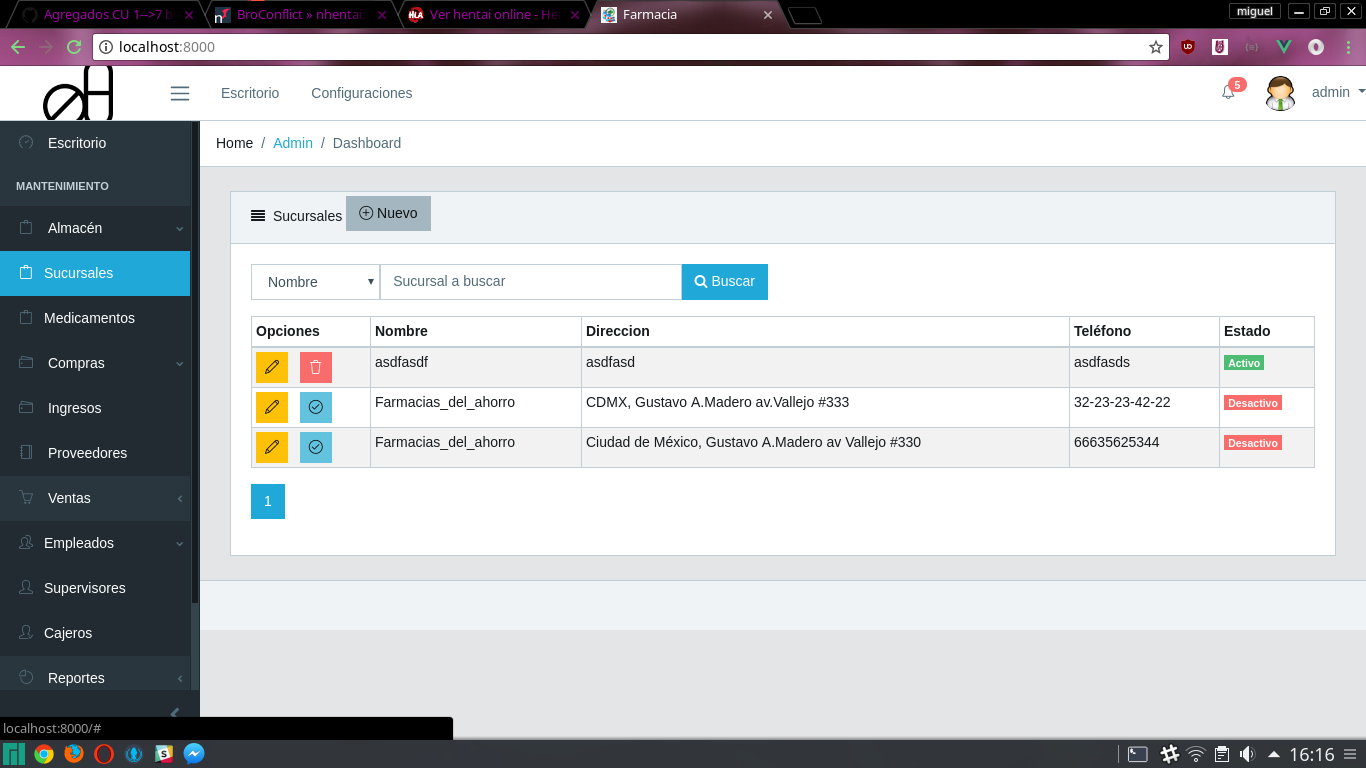
\includegraphics[width=\textwidth]{Pantallas/tablaSucursales}
		\caption{Interfaz de Usuario IU14:Tabla Sucursales.}
	\end{center}
\end{figure}



\begin{figure}[htbp!]
	\begin{center}
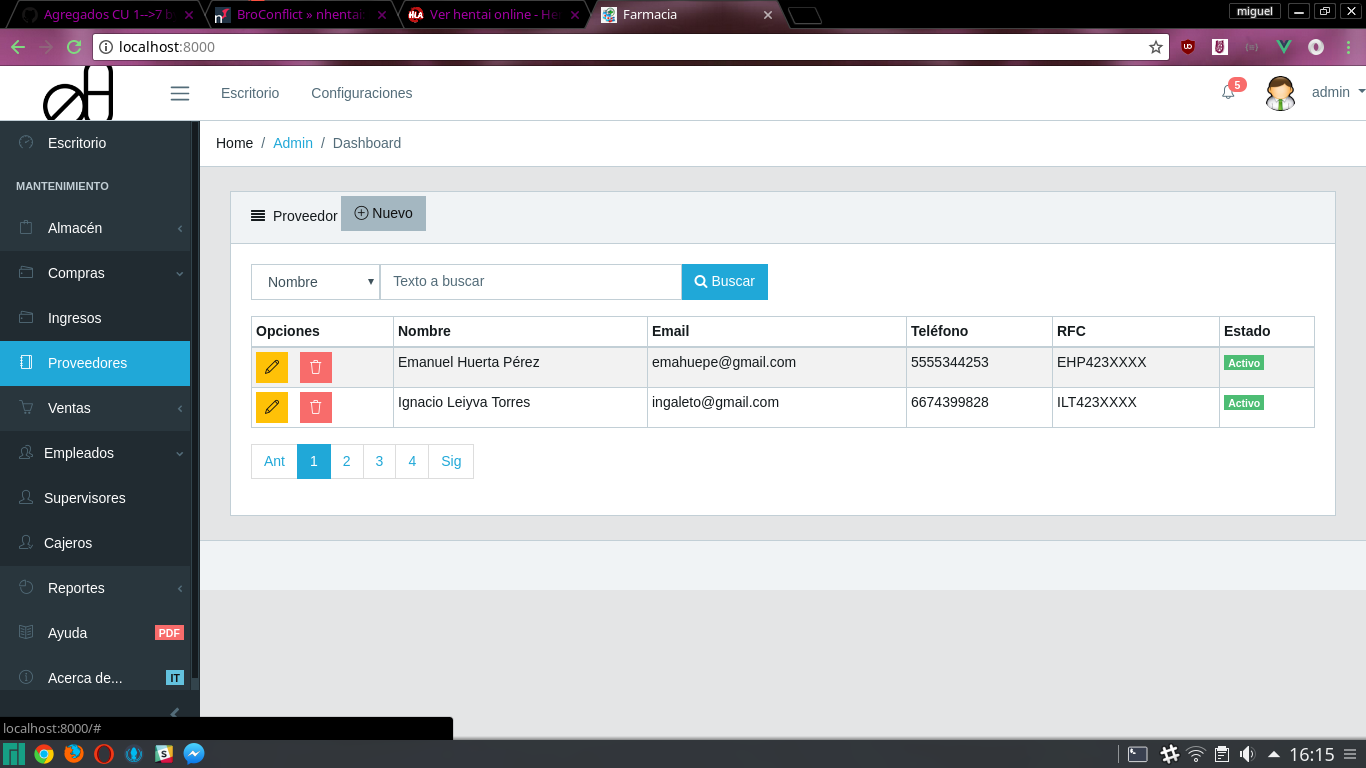
\includegraphics[width=\textwidth]{Pantallas/tablaProveedores}
		\caption{Interfaz de Usuario IU15:Tabla Proveedores.}
	\end{center}
\end{figure}



\begin{figure}[htbp!]
	\begin{center}
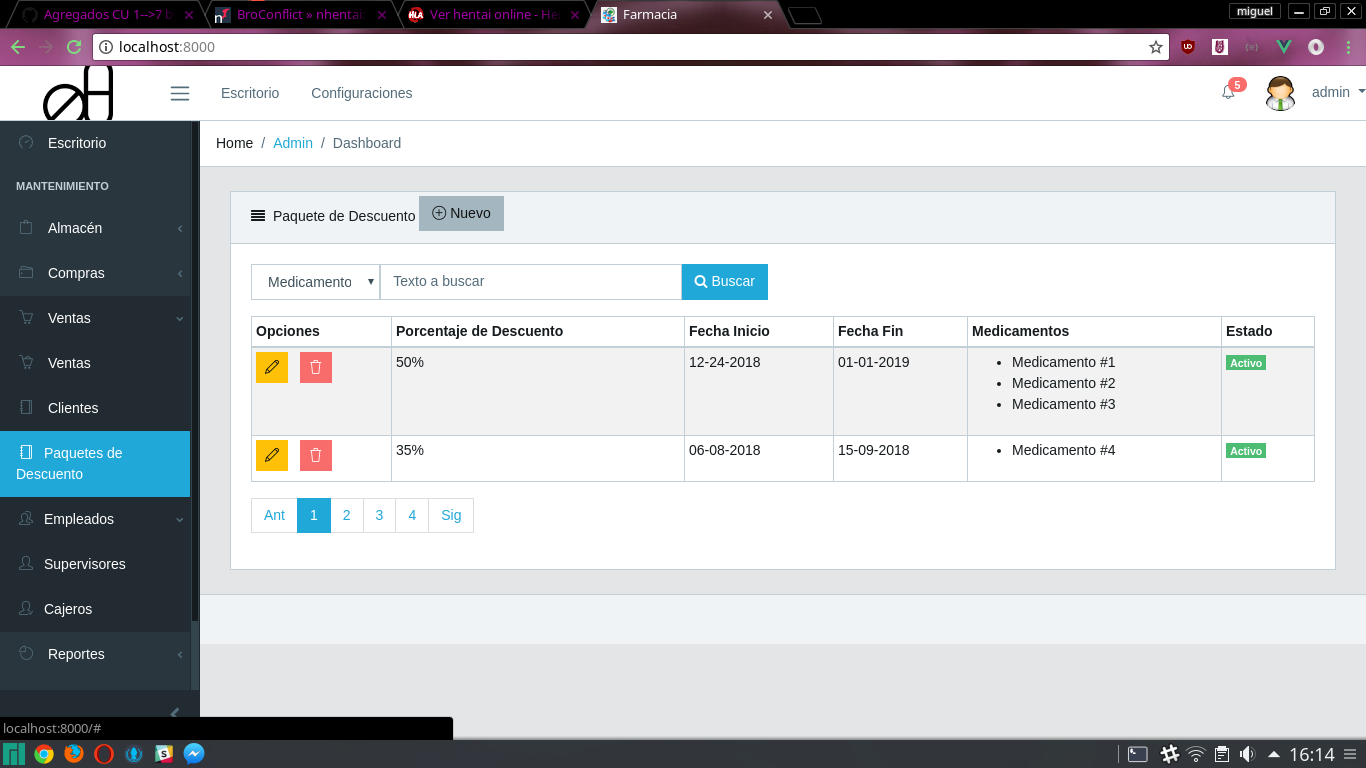
\includegraphics[width=\textwidth]{Pantallas/tablaPaquetesDecuento}
		\caption{Interfaz de Usuario IU16:Tabla Paquetes de Descuentos.}
	\end{center}
\end{figure}



\begin{figure}[htbp!]
	\begin{center}
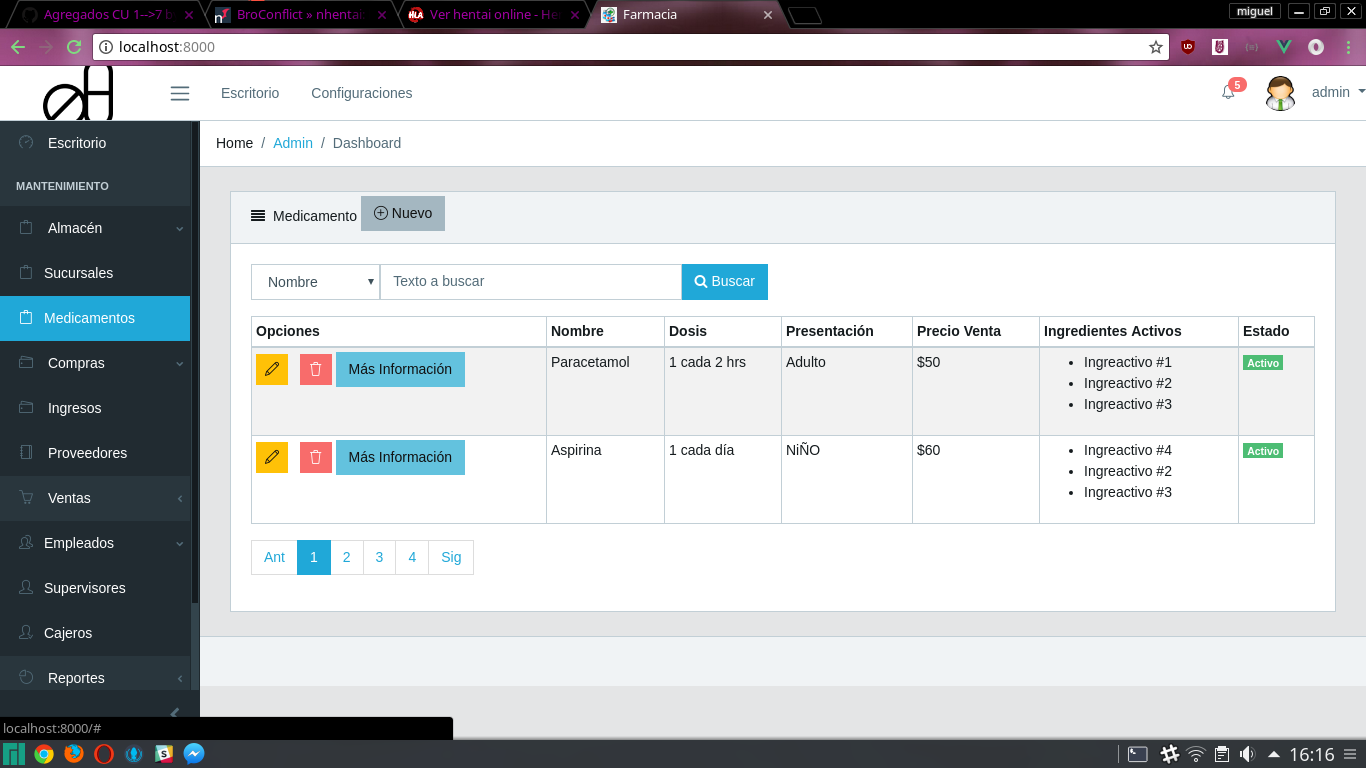
\includegraphics[width=\textwidth]{Pantallas/TablaMedicamentos}
		\caption{Interfaz de Usuario IU17:Tabla Medicamentos.}
	\end{center}
\end{figure}



\begin{figure}[htbp!]
	\begin{center}
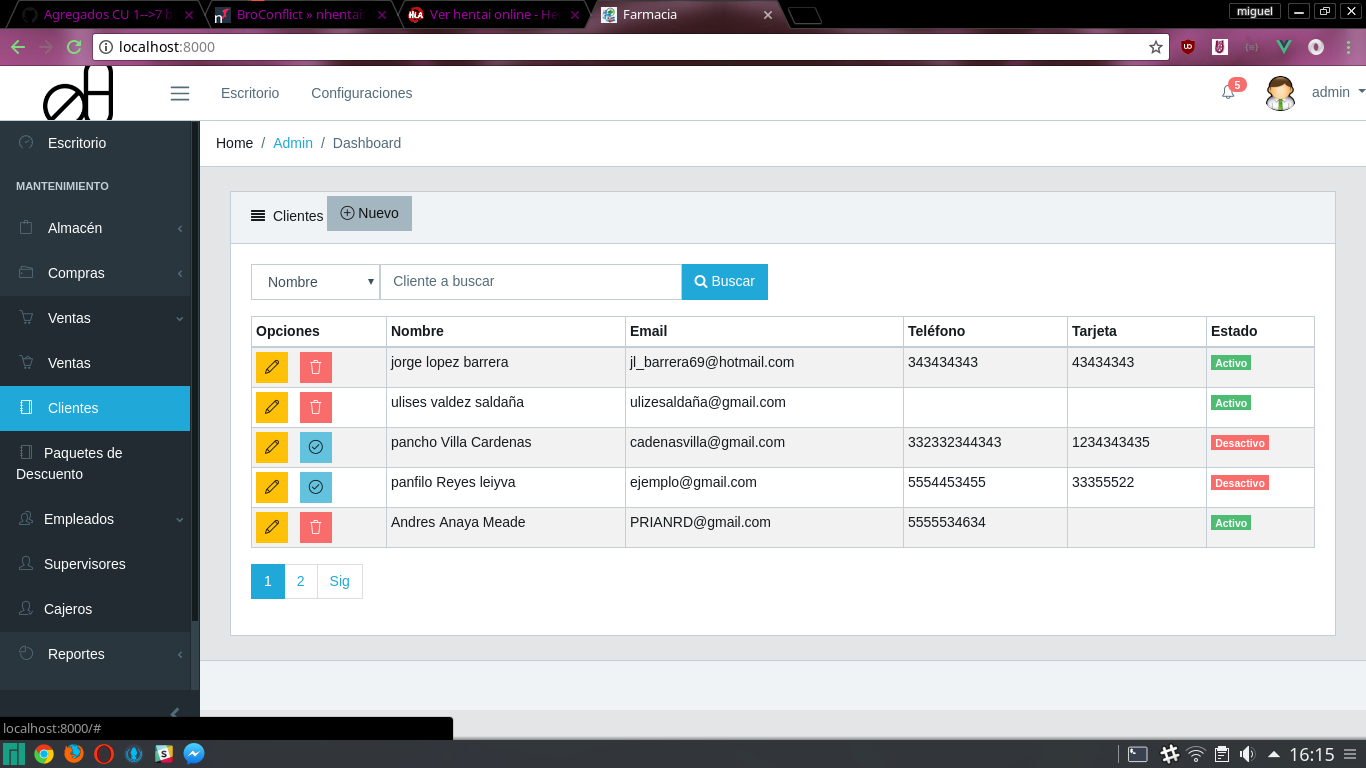
\includegraphics[width=\textwidth]{Pantallas/tablaClientes}
		\caption{Interfaz de Usuario IU18:Tabla Clientes.}
	\end{center}
\end{figure}



\begin{figure}[htbp!]
	\begin{center}
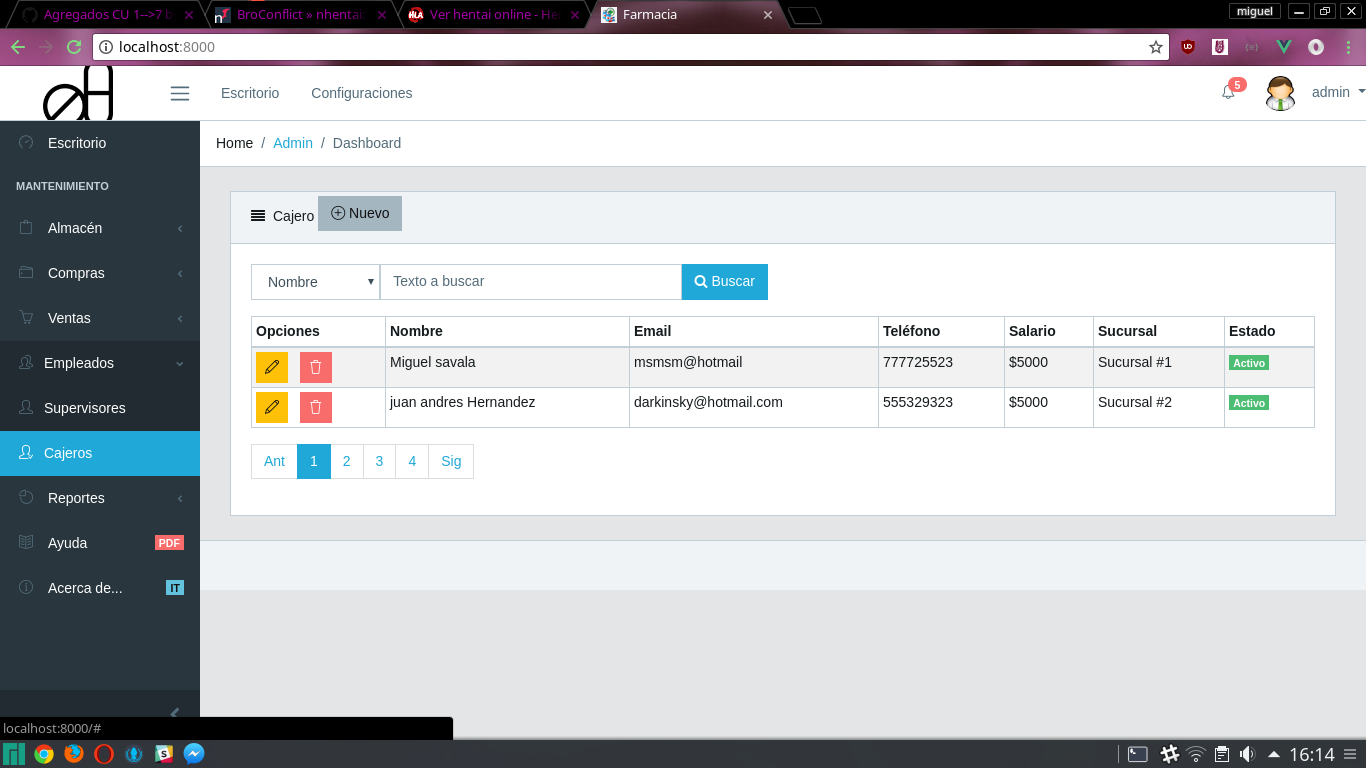
\includegraphics[width=\textwidth]{Pantallas/tablaCajeros}
		\caption{Interfaz de Usuario IU19:Tabla Cajeros.}
	\end{center}
\end{figure}
